%! TeX program = lualatex
\documentclass[ignorenonframetext,aspectratio=169]{beamer}
\usetheme{moloch} % <- change this to your preferred theme
% Add any additional packages you need here:
\usepackage{hyperref}
\usepackage{graphicx}
\usepackage[czech]{babel}
\usepackage{csquotes}
\usepackage{luavlna}
% I use this environment to force linebreaks one source code listing
% that doesn't work well with TeX4ht otherwise. It is redefined in config.cfg. 
% you can remove it if you don't need it.
\newenvironment{likeverbatim}{}{}

\begin{document}
% we must use the \mode command, otherwise \input would be ignored, 
% as the ignorenonframetext option causes all text outside of frames to be ignored
\mode<beamer>{
  % this is the main presentation file, put all slides and accompanying content here
  % if you want to include some content outside of frames also in slides, use \mode<
\mode<beamer|article>{
  \title{Publikace LaTeXových dokumentů na web pomocí TeX4ht a GitHub Actions}
  \author{Michal Hoftich}
  \maketitle
}

\begin{abstract}
Přednáška představí sadu šablon pro nástroj TeX4ht, který slouží k převodu
LaTeXových dokumentů do HTML. Tyto šablony výrazně usnadňují publikaci různých
typů dokumentů na webu a přinášejí moderní možnosti zpracování a automatizace.

První šablona je určena pro převod knižních dokumentů do webové podoby.
Umožňuje rozdělení textu do jednotlivých kapitol s automaticky generovanou
navigací a podporou responzivního designu, takže je výsledek dobře čitelný i na
mobilních zařízeních.

Druhá šablona slouží k tvorbě staticky generovaných blogů. Každý příspěvek je
psán jako samostatný LaTeXový dokument, který je pomocí TeX4ht převeden do
HTML. Následně jsou tyto články zpracovány statickým generátorem webů, jako je
například Jekyll, který se postará o sestavení celého blogu, vytvoření
rozcestníků, archivů a další navigace.

Třetí šablona je zaměřena na převod prezentací vytvořených v prostředí Beamer
do formy tzv. handoutů – přehledových materiálů pro posluchače. Výsledkem je
čitelný a dobře strukturovaný webový dokument vhodný pro sdílení po přednášce.

Všechny šablony jsou navrženy tak, aby fungovaly v rámci GitHub Actions. To
znamená, že dokumenty mohou být automaticky zkompilovány a publikovány online
pokaždé, když dojde ke změně v repozitáři. Tento přístup zajišťuje, že je
webová verze dokumentu vždy aktuální.
\end{abstract}


\tableofcontents

\section{Úvod do TeX4ht}

\begin{frame}{Co je TeX4ht?}
\begin{itemize}
    \item \textbf{Nástroj pro konverzi} z LaTeXu do HTML a dalších formátů (ODT, EPUB, JATS XML)
    \item Zachovává strukturu a formátování původního dokumentu
    \item Podporuje různé metody pro matematický výstup (obrázky, MathML, MathJax)
    \item Umožňuje vytvářet obrázky z výstupu \LaTeX u
    \item Integruje se s běžnými LaTeXovými balíčky
\end{itemize}
\end{frame}

\TeX4ht samotný je především balíček, který redefinuje příkazy jiných balíčků tak, aby
vkládaly tagy výstupních formátů. Vždy se kompiluje do DVI výstupu, který se poté zpracovává
dalšími nástroji, které vytvoří soubory ve výstupním formátu, CSS soubor, nebo obrázky.
Části DVI výstupu lze konvertovat na obrázky ve formátu PNG nebo SVG. To se využívá pro podporu
TikZ nebo PSTricks.

Více informací o \TeX4ht naleznete na  \href{https://www.tug.org/tex4ht/}{oficiálních stránkách}
a v \href{https://www.kodymirus.cz/tex4ht-doc/tex4ht-doc.html}{dokumentaci}.

\begin{frame}[fragile]{Příklad použití TeX4ht}


\begin{block}{Příklad LaTeX kódu}
\begin{verbatim}
Příliš {\bfseries žluťoučký} \textit{kůň}
\end{verbatim}
\end{block}



\begin{block}{Výstup v HTML kódu}
\begin{verbatim}
Příliš <span class='cmbx-10'>žluťoučký </span>
<span class='cmti-10'>kůň</span>
\end{verbatim}
\end{block}

\begin{block}{Výstup v prohlížeči}
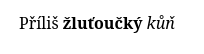
\includegraphics{img/basic.png} 
\end{block}

\end{frame}

V předešlém příkladu \TeX4ht převede LaTeXové příkazy pro tučné a kurzívní písmo na HTML tagy.
Díky tomu, zpracovává DVI soubor, používá informace o použitých fontech a může 
přidat podporu i pro příkazky, které by jinak šly podporovat jen stěží, jako 
\verb|\bfseries| použitý v příkladu.


Pro kompilaci dokumentů pomocí \TeX4ht se používají dva hlavní nástroje: \texttt{make4ht} a \texttt{tex4ebook}.
\texttt{tex4ebook} je starší nástroj, který se používá pro konverzi LaTeXových
dokumentů do formátů pro elektronické knihy, jako je například EPUB.
\texttt{make4ht} vznikl později a je určen pro konverzi LaTeXových dokumentů do
HTML a dalších formátů, jako jsou ODT nebo JATS XML.

\begin{frame}[fragile]{Příklady kompilace pomocí TeX4ht}

\begin{block}{Kompilace do HTML:}
\begin{verbatim}
$ make4ht -ld output_dir soubor.tex
\end{verbatim}
\end{block}



\begin{itemize}
    \item \texttt{-l} - používá Lua\LaTeX\ místo pdf\LaTeX u
    \item \texttt{-d output\_dir} - ukládá výstup do adresáře
\end{itemize}

\begin{block}{Kompilace do EPUB3:}
\begin{verbatim}
$ tex4ebook -f epub3 soubor.tex
\end{verbatim}
\end{block}

\begin{itemize}
    \item \texttt{-f epub3} - specifikuje formát EPUB3
\end{itemize}
\end{frame}

\begin{frame}[fragile]{Konfigurace výstupního formátu}
\begin{block}{Konfigurační soubor pro \TeX4ht}
\begin{verbatim}
\Preamble{xhtml}
\Configure{textit}{\HCode{<i>}\NoFonts}{\EndNoFonts\HCode{</i>}}
\begin{document}
\EndPreamble
\end{verbatim}
\end{block}

\begin{block}{Kompilujeme pomocí:}
\begin{verbatim}
$ make4ht -c config.cfg soubor.tex
\end{verbatim}
\end{block}

\begin{block}{HTML výstup}
\begin{verbatim}
Příliš <span class='cmbx-10'>žluťoučký </span><i>kůň</i>  
\end{verbatim}
\end{block}
\end{frame}

Konfigurační soubor  umožňuje redefinovat výstup
pro příkazy podporované \TeX4ht. V tomto příkladu
se jmenuje \texttt{config.cfg} a voláme ho pomocí volby \texttt{-c}.
Příkaz \verb|\Configure| umožňuje vkládat obsah do háčků, definovaných v 
konfiguračních souborech \TeX4ht pro jednotlivé balíčky. 

V tomto případě využíváme konfiguraci pro \texttt{textit}, která využívá
dva háčky -- jeden vkládá před obsah příkazu \verb|\textit|, druhý za něj.
Tagy vkládáme pomocí příkazu \verb|\HCode|. Abychom zabránili vložení tagů
\verb|<span>| pro aktuální font, použijeme příkaz \verb|\NoFonts|, který 
vypíná zpracování fontů. Na konci konfigurace je třeba opět zpracování fontů
zapnout pomocí \verb|\EndNoFonts|.

\begin{frame}[fragile]{Struktura konfiguračního souboru}
\begin{verbatim}
\Preamble{xhtml,<volby tex4ht>}
<konfigurace>
\begin{document}
<pozdní konfigurace>
\EndPreamble
\end{verbatim}
\end{frame}

Více informací o konfiguračních souborech \TeX4ht naleznete v kapitole
\href{https://www.kodymirus.cz/tex4ht-doc/Configurations.html}{o konfiguracích}
v dokumentaci \TeX4ht.

\begin{frame}[fragile]{Volby pro \TeX4ht}

\begin{block}{}
\begin{verbatim}
$ make4ht soubor.tex "mathml,mathjax"
\end{verbatim}
\begin{itemize}
  \item Volby můžeme zadat jako řetězec v uvozovkách
  \item Další možností je použít příkaz \verb|\Preamble| v konfiguračním souboru
\end{itemize}
\end{block}

\begin{block}{Příklady voleb}
\begin{itemize}
  \item \texttt{mathml} – generuje MathML pro matematické výrazy
  \item \texttt{mathjax} – používá MathJax pro zobrazení matematiky
  \item \texttt{pic-m} - vytváří obrázky pro inline matematiku
  \item \texttt{svg} – generuje SVG obrázky pro TikZ nebo PSTricks
\end{itemize}
\end{block}
\end{frame}

\begin{frame}[fragile]{Rozšíření pro make4ht}
\begin{block}{Povolení rozšíření}
\begin{verbatim}
$ make4ht -f html5+název_rozšíření soubor.tex
\end{verbatim}
\end{block}
\begin{block}{Zakázání rozšíření}
\begin{verbatim}
$ make4ht -f html5-název_rozšíření soubor.tex 
\end{verbatim}
\end{block}



\begin{block}{Příklady rozšíření}
\begin{itemize}
\item \verb|dvisvgm_hashes| -- pro efektivní vytváření SVG obrázků
\item \verb|common_domfilters| -- oprava HTML výstupu pomocí LuaXML
\item \verb|staticsite| -- pro vytvoření souborů ve formátu vhodném pro generátory statických webů
\end{itemize}
\end{block}

\end{frame}

Rozšíření umožňují přizpůsobit chování \TeX4ht pro specifické potřeby. Většinou upravují výstupní soubory
produkované \TeX4ht, například  upravují strukturu HTML dokumentu. 

Rozšíření se povolují nebo zakazují pomocí znamének plus a minus za názvem výstupního formátu. 
Můžeme jich povolit více najednou, například \verb|html5+staticsite+dvisvgm_hashes|.
Některá rozšíření, například \verb|common_domfilters|, jsou povolena implicitně, ale mohou být vypnuta pomocí znaménka minus.

\begin{frame}[fragile]{Build soubory pro TeX4ht}

\begin{block}{Úprava CSS souboru}
\begin{verbatim}
local filter = require("make4ht-filter")  
local process = filter {  
  function(text)  
    -- Nahrazení písma v CSS  
    return text:gsub("TeXGyreTermesX", "Georgia")  
  end  
}  
Make:match("css", process)  -- Aplikuje filtr na CSS soubory
\end{verbatim}
\end{block}

\begin{block}{Použití v make4ht}
\begin{verbatim}
$ make4ht -e build.lua soubor.tex
\end{verbatim}
\end{block}
\end{frame}

Build soubory jsou Lua skripty, které upravují kompilační proces. Například 
v nich můžeme upravovat výstupní soubory. V předešlé ukázce využíváme 
knihovnu \texttt{make4ht-filter} pro úpravu CSS souboru. Pomocí filtru 
můžeme definovat funkce, které upraví text daného souboru. Funkce můžeme řetězit.
V této ukázce nahrazujeme písmo \texttt{TeXGyreTermesX} za \texttt{Georgia} v CSS souboru.
Filtr poté aplikujeme na všechny CSS soubory pomocí příkazu \texttt{Make:match("css", process)}.

\begin{frame}[fragile]{Úprava kompilačního procesu}
\begin{block}{Volání programu Xindex}
\begin{verbatim}
Make:htlatex {} 
Make:xindex {} 
Make:autohtlatex {}
\end{verbatim}
\end{block}

\end{frame}

V build souborech můžeme také volat další programy, které se mají spustit. V \texttt{make4ht}
jsou definovány různé funkce, které je spouští. Například \texttt{Make:htlatex} spustí
jednu kompilaci pomocí \LaTeX u, \texttt{Make:xindex} spustí program \texttt{xindex}
a \texttt{Make:autohtlatex} spustí kompilaci \LaTeX em s automatickou detekcí počtu kompilací
nutných k tomu, aby správně fungovaly křížové odkazy nebo tabulky. Ty totiž potřebují více než jednu kompilaci, k tomu
aby se správně vytvořily.


\section{Využití Githubu pro automatické publikování}

\begin{frame}[fragile]{Použití šablony na GitHubu}
  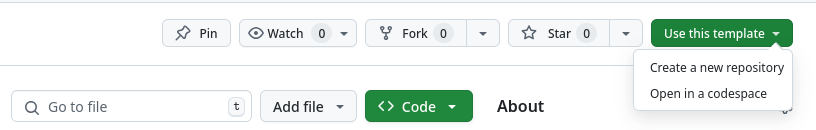
\includegraphics[width=\textwidth,alt={}]{img/template-use.png}
\end{frame}

Pro využití šablon na Githubu klikněte na tlačítko
\enquote{Use this template} na stránce GitHub repozitáře s podporou šablon. 

Tím se ve vašem účtu vytvoří
nový repozitář se stejnou strukturou a soubory. Poté jej můžete naklonovat,
upravit obsah a začít vytvářet vlastní snímky a handouty.

\begin{frame}[fragile]{Vytvoření nového GitHub repozitáře}
  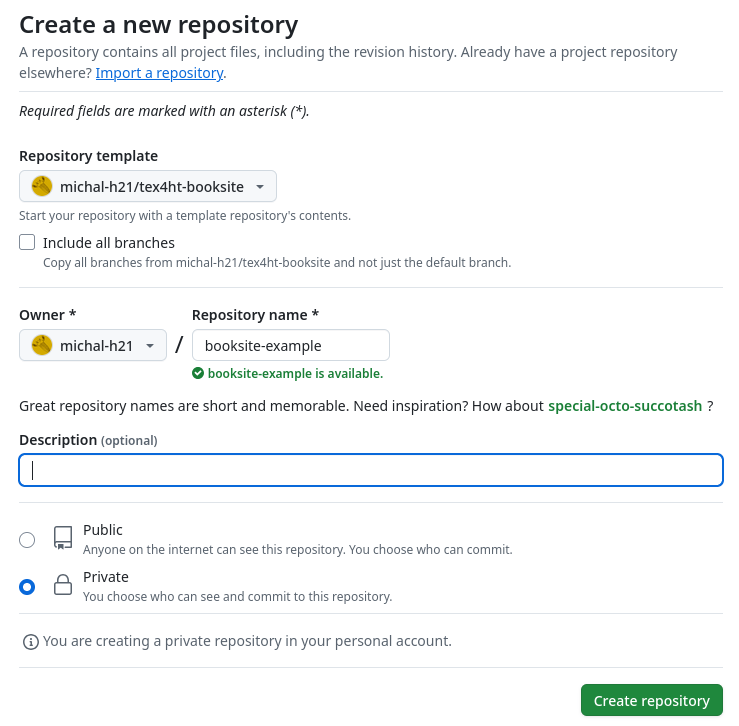
\includegraphics[width=0.6\textwidth,alt={Dialog vytvoření nového repozitáře ze šablony}]{img/new-repo.png}
\end{frame}

Po 

% \subsection{Github Actions}

\begin{frame}[fragile]{Rozhraní Github Actions}
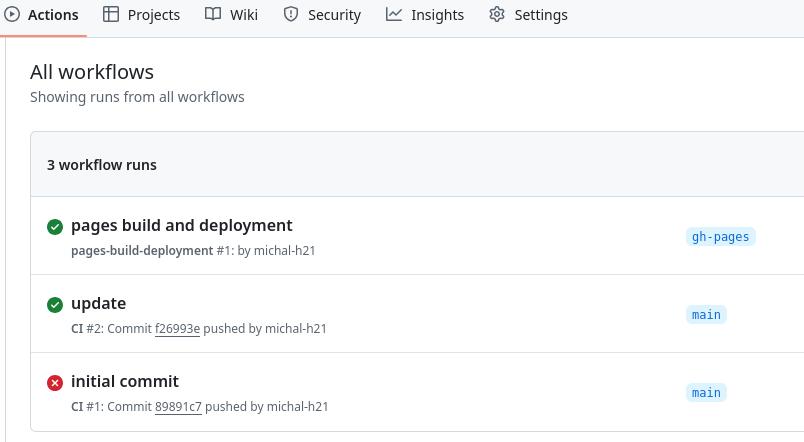
\includegraphics[width=\textwidth]{img/github-actions.png}
\end{frame}

Po pushnutí změn do větve \texttt{main} můžete zkontrolovat záložku
\texttt{Actions} ve vašem Github repozitáři. Zobrazuje stav workflow, včetně
informace o úspěšném dokončení nebo případných chybách.

\begin{frame}[fragile]{Chyby}
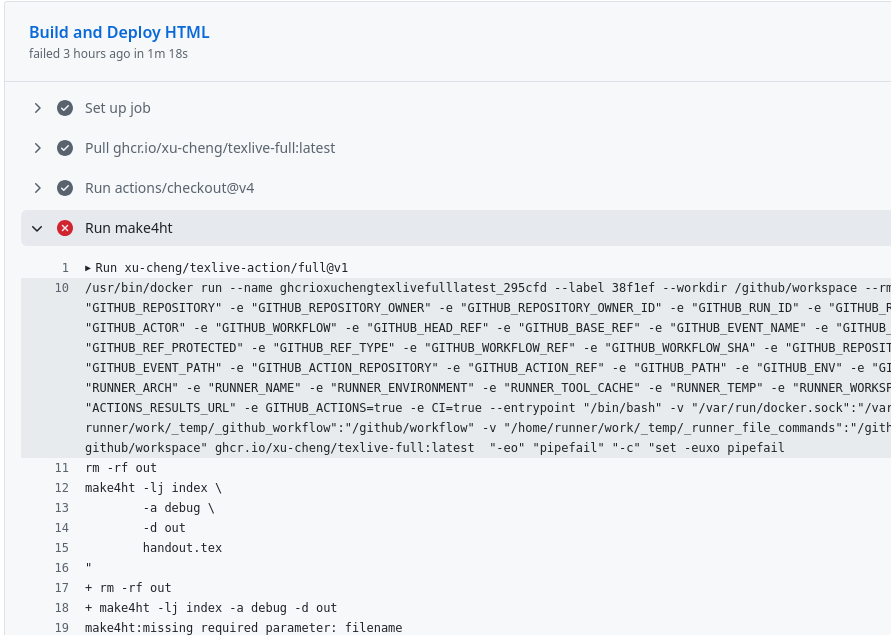
\includegraphics[width=\textwidth]{img/github-error.png}
\end{frame}

Můžete také zkontrolovat logy běhu workflow, abyste viděli, co se pokazilo.
Pokud narazíte na chybu, bude zobrazena v logu a můžete tyto informace
použít k řešení problému.

V tomto případě byl nesprávný název TeX souboru. Musel jsem opravit název
souboru v YAML souboru GitHub Actions.

% \subsection{Publikování HTML verze}

\begin{frame}[fragile]{Nastavení Github Pages}
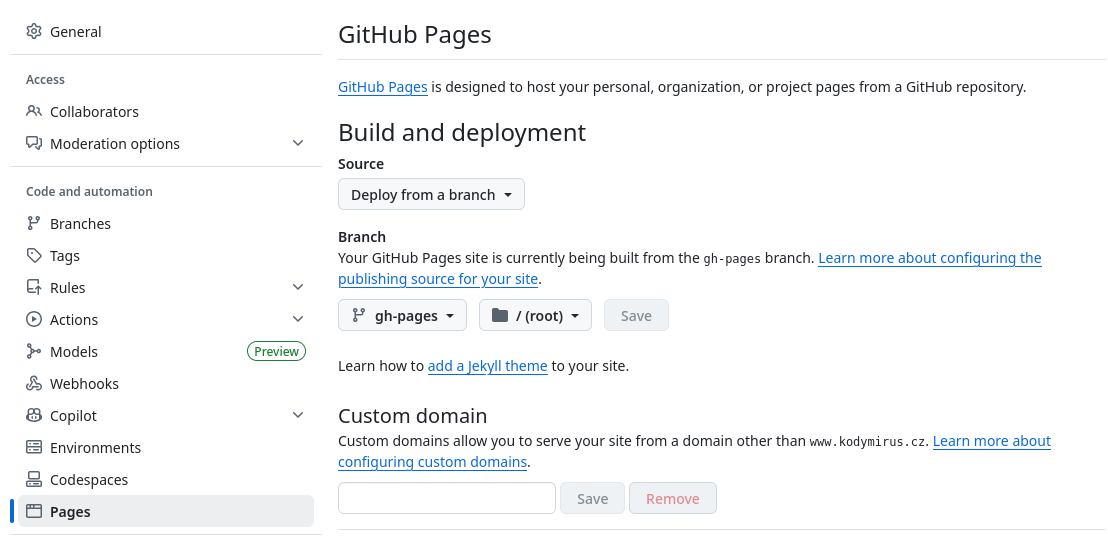
\includegraphics[width=\textwidth]{img/github-pages.png}
\end{frame}

Po úspěšném dokončení workflow můžete nastavit GitHub Pages pro zobrazování obsahu větve \texttt{gh-pages}.

Všechny výstupní soubory vytvořené pomocí \texttt{make4ht} budou dostupné na webu.
Budou přístupné na adrese:
\verb|https://username.github.io/repo/|,
kde \texttt{username} je vaše GitHub uživatelské jméno a \texttt{repo} je název vašeho repozitáře.

Například příklady použité v této prezentaci naleznete na adresách \url{https://michal-h21.github.io/tex4ht-presentation/},
\url{https://michal-h21.github.io/tex4ht-booksite/}

\section{Šablona pro prezentace}

Tato šablona je určena pro prezentace, které potřebují víc než jen snímky. Umožňuje vytvořit jak samotnou prezentaci, tak podrobný handout s poznámkami a komentáři. Všechny materiály tak lze generovat z jednoho zdrojového souboru – jak pro živou prezentaci, tak pro lidi, kteří se prezentace neúčastnili.

Obsahuje několik hlavních zdrojových souborů, každý s konkrétním účelem:

\begin{frame}[fragile]{Přehled souborů}
\begin{itemize}
\item \textbf{\texttt{slides.tex}}
\item \textbf{\texttt{handout.tex}}
\item \textbf{\texttt{presentation.tex}}
\item \textbf{\texttt{preamble.tex}}
\item \textbf{\texttt{config.cfg}}
\end{itemize}
\end{frame}

\begin{itemize}
\item \textbf{\texttt{slides.tex}} – Tento soubor slouží ke generování hlavní prezentace ve formátu Beamer. Obsahuje to, co se zobrazuje během přednášky.

\item \textbf{\texttt{handout.tex}} – Handoutová verze prezentace, formátovaná jako standardní článek. Kromě obsahu viditelného na snímcích obsahuje i doplňující poznámky a komentáře, které se v samotné prezentaci nezobrazují. Tento soubor je určen ke sdílení po skončení prezentace a měl by být samostatně použitelný i pro čtenáře, kteří prezentaci neviděli.

\item \textbf{\texttt{presentation.tex}} – Obsahuje celý zdrojový text prezentace. Obsah uvnitř prostředí \verb|\begin{frame}...\end{frame}| se zahrnuje jak do \texttt{slides.tex}, tak do \texttt{handout.tex}. Text mimo prostředí frame se v prezentaci nezobrazí, ale je součástí handoutu. To umožňuje doplnit prezentaci o podrobnější komentáře, vysvětlení nebo poznámky.

\item \textbf{preamble.tex} – Obsahuje balíčky a definice příkazů používané v prezentaci.

\item \textbf{config.cfg} – Konfigurační soubor pro \TeX4ht. Například zde můžete upravit CSS styly použité ve webové verzi dokumentu nebo redefinice \LaTeX{}ových příkazů.
\end{itemize}

Tyto soubory si můžete upravit podle svých potřeb. Minimálně je vhodné nahradit obsah \texttt{presentation.tex} vlastním textem a případně upravit \texttt{preamble.tex}, pokud potřebujete přidat další balíčky nebo příkazy.

\subsection{Základní použití}


\begin{frame}[fragile]{Použití prostředí frame a komentáře v handoutu}

\begin{block}{}
Základní syntaxe dokumentu používaného v souboru \verb|presentation.tex| vypadá následovně:
\end{block}

\begin{likeverbatim}\verb|\begin{frame}{Název snímku}|\
\verb|obsah snímku...|\
\verb|\end|\verb|{frame}|\
\vspace{1em}
\verb|Komentář, který bude zahrnut pouze v handoutu|
\end{likeverbatim}

\end{frame}

Například zdrojový kód jednoho z předchozích snímků vypadá takto:

\verb|\begin|\verb|{frame}[fragile]{Přehled souborů}|
\begin{verbatim}
\begin{itemize}
\item \textbf{\texttt{slides.tex}}
\item \textbf{\texttt{handout.tex}}
\item \textbf{\texttt{presentation.tex}}
\item \textbf{\texttt{preamble.tex}}
\end{itemize}
\end{verbatim}
\verb|\end|\verb|{frame}|

\begin{verbatim}
\begin{itemize}
\item \textbf{\texttt{slides.tex}} – Tento soubor slouží ke generování hlavní
prezentace ve formátu Beamer. Obsahuje to, co se zobrazuje během přednášky.
\end{itemize}
\end{verbatim}

Obsah uvnitř bloku \verb|\begin|\verb|{frame}...\end|\verb|{frame}| se zahrne
do prezentace i handoutu, ale prostředí \texttt{itemize}, které následuje za
ním, se zobrazí pouze v handoutu.

\begin{frame}[fragile]{Sdílený obsah mimo prostředí frame}

\begin{verbatim}
\mode<beamer|article>{
\title{Strukturovaná šablona prezentace}
\author{Michal Hoftich}
\maketitle
}
\end{verbatim}
\end{frame}

Příkaz \verb+\mode<beamer|article>{...}+ umožňuje zahrnout obsah, který se má
zobrazit jak v prezentaci, tak v handoutu. To se může hodit například pro název
prezentace nebo obsah prezentace.

\subsection{Kompilace prezentace}

\begin{frame}[fragile]{Kompilace do PDF}

Prezentaci nebo handout můžete zkompilovat do PDF pomocí LuaLaTeXu těmito příkazy:

\begin{verbatim}
$ lualatex slides.tex
$ lualatex handout.tex
\end{verbatim}
\end{frame}



Výstupní soubory můžete kompilovat v libovolné standardní distribuci \LaTeX{}u, která obsahuje Beamer a potřebné balíčky.

\begin{frame}[fragile]{HTML verze}
Pro převod prezentace do formátu HTML použijte nástroj \href{https://www.tug.org/tex4ht/}{\TeX4ht}.
\begin{verbatim}
$ make4ht -l handout.tex\end{verbatim}

Přepínač \verb|-l| zajistí použití Lua\LaTeX{}u jako překladače.
\end{frame}

HTML verze se generuje z handoutu ve stylu článku, nikoliv z Beamer prezentace.
To ji činí vhodnější pro webové publikování nebo dlouhodobé sdílení, protože
obsahuje všechny vysvětlivky a není závislá na rozvržení snímků.

section{Automatické generování HTML výstupu}

Tato část vysvětluje, jak se používají \href{https://docs.github.com/en/actions/writing-workflows/quickstart}{GitHub Actions} k automatickému generování a publikování HTML verze materiálů při každém pushnutí změn do větve \texttt{main}.

Výstup je vytvářen pomocí \texttt{make4ht} a publikován do větve \texttt{gh-pages}, což usnadňuje sdílení webové verze prezentace.

\begin{frame}[fragile]{Přehled GitHub Actions}
Klíčové části workflow pro sestavení a publikování HTML:

\begin{verbatim}

    name: Spuštění make4ht
    uses: xu-cheng/texlive-action/full@v1
    with:
      run: |
      make4ht -lj index -a debug -d out handout.tex

    name: Publikování webových stránek
    uses: peaceiris/actions-gh-pages@v3
    with:
      github_token: ${{ secrets.GITHUB_TOKEN }}
      publish_dir: ./out
\end{verbatim}

\end{frame}

Workflow je definován v souboru \texttt{.github/workflows/main.yml}.
Tento soubor můžete upravit pro přizpůsobení procesu sestavení, například změnou parametrů pro \texttt{make4ht}.

Používají se dvě GitHub Actions: \href{https://github.com/xu-cheng/texlive-action}{xu-cheng/texlive-action}
a \href{https://github.com/peaceiris/actions-gh-pages}{peaceiris/actions-gh-pages}.
První umožňuje používat libovolný příkaz dostupný v TeX Live instalaci, jako \texttt{make4ht} nebo \texttt{lualatex}.
Druhá publikuje obsah zadaného adresáře do větve \texttt{gh-pages} vašeho repozitáře,
kterou GitHub Pages používá pro zobrazování statického obsahu.

\begin{frame}[fragile]{Automatické sestavení HTML}
Změny pushnuté do větve \texttt{main} spustí GitHub Actions workflow, který:

\begin{itemize}
\item Zkompiluje \texttt{handout.tex} do HTML pomocí \texttt{make4ht}
\item Publikuje výstup do větve \texttt{gh-pages}
\end{itemize}

Použitý příkaz je:

\begin{verbatim}
make4ht -lj index -a debug -d out handout.tex
\end{verbatim}
\end{frame}

Tento příkaz vytvoří HTML soubory v adresáři \texttt{out/}, které jsou následně publikovány
pomocí akce \texttt{peaceiris/actions-gh-pages}, specifikované nastavením
\texttt{publish_dir}.

\begin{frame}[fragile]{Proč \texttt{-j index}?}
\begin{itemize}
\item Volba \texttt{-lj index} je zkratka pro \texttt{-l -j index}
\item Volba \texttt{-j index} nastaví název výstupního HTML souboru na \texttt{index.html}
\item To umožňuje používat čisté URL adresy jako:

\begin{verbatim}
https://username.github.io/repo/
\end{verbatim}

\end{itemize}
\end{frame}

Není potřeba v URL specifikovat název souboru - GitHub Pages
automaticky hledá soubor \texttt{index.html}. Toto usnadňuje sdílení
prezentace a pomáhá předejít nefunkčním odkazům kvůli neshodě názvů souborů.



}
\end{document}


